%!TEX root = ../thesis.tex

本章では, 先行研究を基にした提案手法をデータの収集方法, 訓練, 実験の3節に分けて紹介する.

\section{手法1}

\subsection{データの収集方法}
\figref{Fig:old-method}にデータの収集方法を示す. 赤色の線である目標経路から平行に±0.10, ±0.20, ±0.30m離れた座標にロボットを配置する. そして, その座標ごとに目標経路に沿った向きを基準として±5度傾けて, 64×48のカメラ画像(RGB画像)とルールベース制御器によるナビゲーションの出力である角速度を\figref{Fig:collect-data2}のように収集する. これをGazeboのWillow Garageで\figref{Fig:willow-garage}に示すコースで一周行う.

% \vspace{10mm}

\begin{figure}[h]
  \centering
  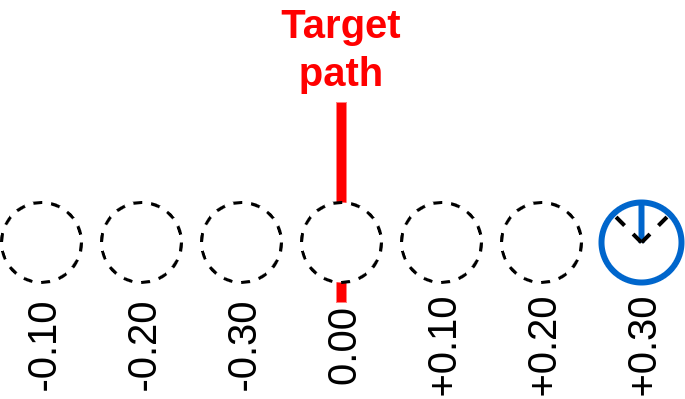
\includegraphics[keepaspectratio, scale=0.25]{images/old-method.png}
  \caption{Method of collecting data around the target route}
  \label{Fig:old-method}
  \end{figure}

\newpage
  \begin{figure}[h]
  \centering
  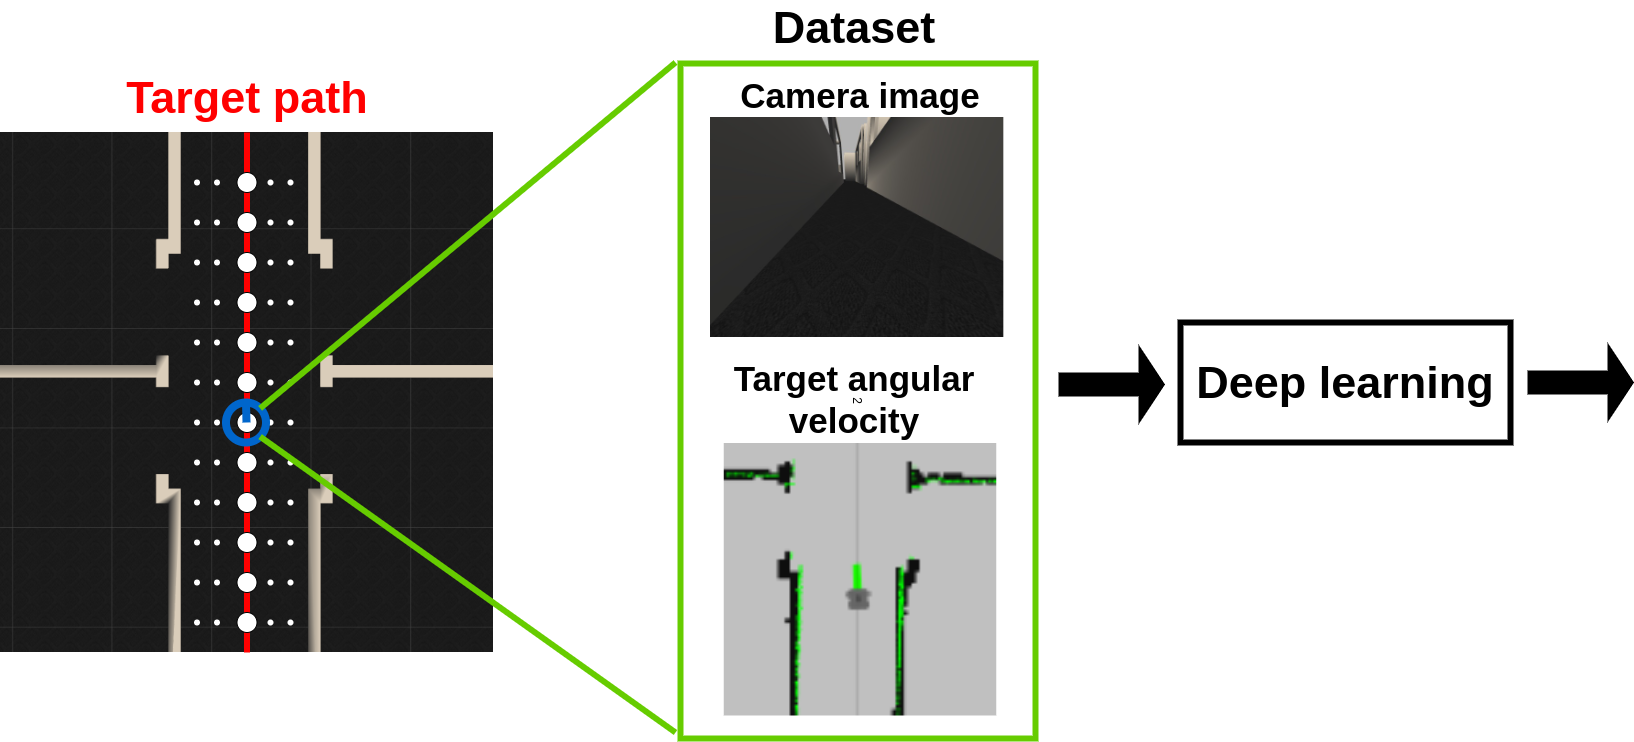
\includegraphics[keepaspectratio, scale=0.25]{images/collect-data2.png}
  \caption{Method of collecting data around the target route}
  \label{Fig:collect-data2}
  \end{figure}

\vspace{15mm}

\begin{figure}[h]
  \centering
  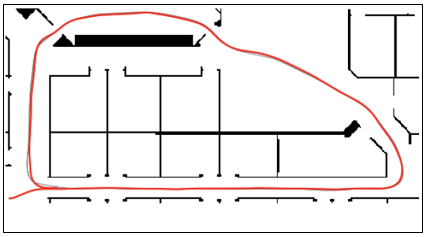
\includegraphics[keepaspectratio, scale=0.5]{images/willow-garage.png}
  \caption{Course to collect data}
  \label{Fig:willow-garage}
  \end{figure}

\newpage
\subsection{訓練1}
\paragraph{ネットワークの構造}
\figref{Fig:cnn}に訓練時に用いたネットワークの構造を示す. 構造は, 入力層1, 畳み込み層3, 全結合層2, 出力層1の計7層から構成されている. 以下, ネットワークの構造は同じである. 

\vspace{5mm}
\begin{figure}[h]
  \centering
  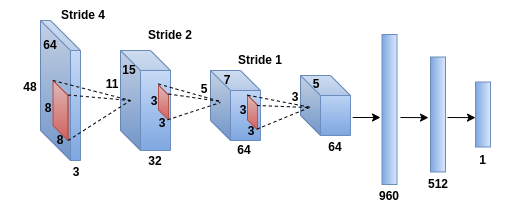
\includegraphics[keepaspectratio, scale=0.6]{images/cnn.png}
  \caption{Structure of network}
  \label{Fig:cnn}
  \end{figure}

\paragraph{訓練}
バッチサイズ8, データ量2658, ミニバッチ学習(先行研究に倣って)で4000step, 8000step, 10000step学習した.

\subsection{実験1}
\paragraph{実験目的}
シミュレータ上で実験を行い, 提案手法の有効性を検証する.

\paragraph{実験装置}
シミュレータを用いた実験では, データの収集方法と同様にWillow Garageを使用した. また, ロボットモデルには\figref{Fig:turtlebot3}に示すようなカメラを3つ搭載したTurtlebot3を用いた. 

\begin{figure}[h]
  \centering
  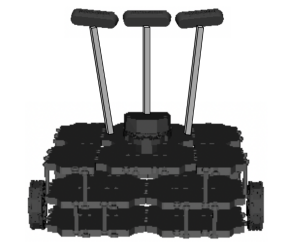
\includegraphics[keepaspectratio, scale=0.55]{images/turtlebot3.png}
  \caption{Turtlebot3 waffle with 3 cameras}
  \label{Fig:turtlebot3}
  \end{figure}

\newpage
\paragraph{実験方法}
シミュレータを用いた実験では, \figref{Fig:willow-garage}で示した経路で実験を行う. 壁に衝突せずに一周できた場合を成功とし, 壁に激突したり, コースアウトして経路に復帰できなかった場合を失敗とした. \par ※以下, 実験目的, 実験装置, 実験方法は同じである. 

\paragraph{実験結果}
実験結果は, \ref{tb:exp1}, 失敗箇所は\figref{Fig:result1}のようになった. 青色の×は壁への衝突箇所を示している. 

\begin{table}[h]
  \centering
  \begin{tabular}{|c|c|} \hline
    step & Number of successes \\ \hline
    4000 & 0/10 \\ \hline
    8000 & 0/10 \\ \hline
    10000 & 0/10 \\ \hline
  \end{tabular}
  \caption{Number of successes in the experiment1}
  \label{tb:exp1}
\end{table}

\begin{figure}[h]
  \centering
  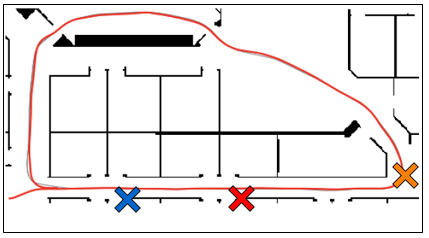
\includegraphics[keepaspectratio, scale=0.5]{images/result1.png}
  \caption{Failure point of the experiment1}
  \label{Fig:result1}
  \end{figure}

\newpage
\paragraph{考察}
学習量を増やしても成功回数は増えなかった.  また, 目標経路から離れた際に戻る挙動や, 壁に近づきすぎた際に避ける挙動も見られなかった. そこで, 収集した角速度を\figref{Fig:exp1}のようにヒストグラムにした. これより, 経路上及び経路周辺のデータ(0から0.1)が全体の40%程度しかないことが分かる. 経路上及び経路周辺のデータが多い方が, 経路追従の成功回数が増えるのではないかと考えた. 

\begin{figure}[h]
  \centering
  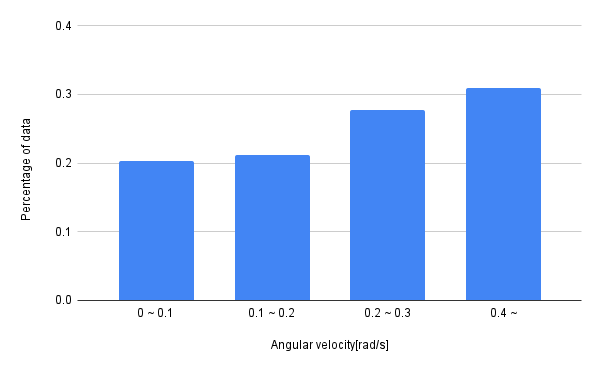
\includegraphics[keepaspectratio, scale=0.6]{images/exp1.png}
  \caption{Histogram of collected angular velocities in the experiment1}
  \label{Fig:exp1}
  \end{figure}

\newpage
\section{手法2}

\subsection{データの収集方法}
手法1を踏まえて, 経路周辺のデータを多く取得する手法を試みる. \figref{Fig:collect-data}にデータの収集方法を示す. 赤色の線である目標経路から平行に±0.01, ±0.02, ±0.04, ±0.06, ±0.08, ±0.10, ±0.15, ±0.20, ±0.30m離れた座標にロボットを配置する. そして, 手法1と同様にロボットを傾けて画像と角速度を\figref{Fig:collect-data2}のように収集する. これを\figref{Fig:willow-garage}に示すコースで一周行う. 

\begin{figure}[h]
  \centering
  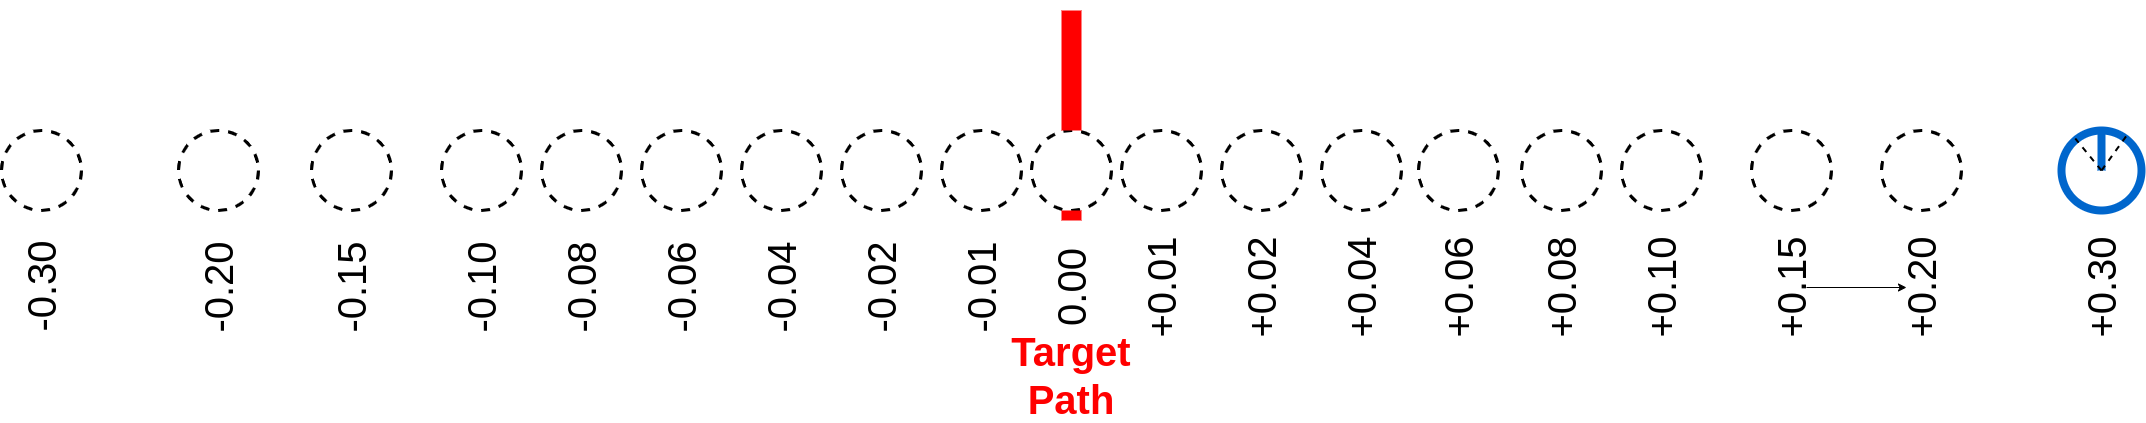
\includegraphics[keepaspectratio, scale=0.18]{images/collect-data.png}
  \caption{Method of collecting data around the target route}
  \label{Fig:collect-data}
  \end{figure}

\vspace{15mm}
\subsection{訓練2-1} 

\paragraph{訓練}
バッチサイズ8, データ量7242, ミニバッチ学習で4000step, 8000step, 10000step学習した.

\subsection{実験2-1}

\paragraph{実験結果}
実験結果は, \ref{tb:exp2}のようになった. \figref{Fig:result2}の青×の箇所でコースアウトして, 目標経路に復帰できなかった. 

\begin{table}[h]
  \centering
  \begin{tabular}{|c|c|} \hline
    step & Number of successes \\ \hline
    4000 & 0/10 \\ \hline
    8000 & 0/10 \\ \hline
    10000 & 0/10 \\ \hline
  \end{tabular}
  \caption{Number of successes in the experiment2-1}
  \label{tb:exp2}
\end{table}

\begin{figure}[h]
  \centering
  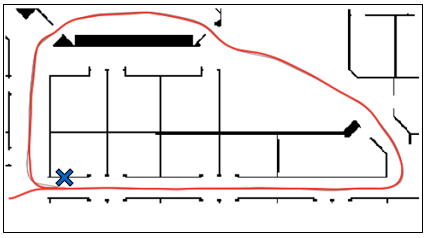
\includegraphics[keepaspectratio, scale=0.6]{images/result2.png}
  \caption{Failure point of the experiment2-1}
  \label{Fig:result2}
  \end{figure}

\newpage
\paragraph{考察}
収集した角速度を\figref{Fig:exp2}のようにヒストグラムにした. 経路上及び経路周辺のデータが\figref{Fig:exp1}と比べて多くなっている. これにより, \figref{Fig:result2}の青枠の区間において, 壁に衝突することなく走行できていることが分かる. しかし, データ量や学習量を変化させても成功回数は増えなかった. そこで, 先行研究のオンライン学習では計算のリソースなどの観点からミニバッチ学習にしていたが, 提案手法ではオフラインで学習を行うため, バッチ学習に変更する. これにより, 一度に大量のデータを扱えるため最適解に辿り着くことができ, 成功回数が増えるのではないかと考えた. 

\begin{figure}[h]
  \centering
  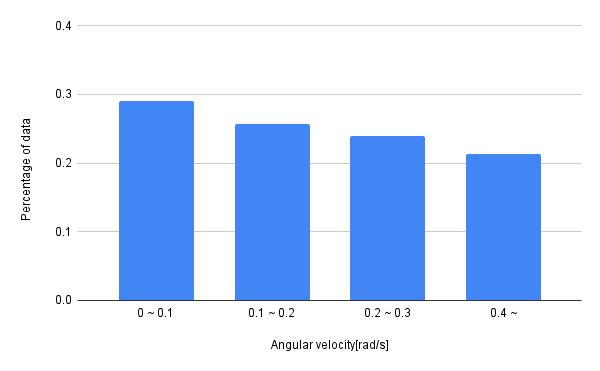
\includegraphics[keepaspectratio, scale=0.6]{images/exp2.png}
  \caption{Histogram of collected angular velocities in the experiment2-1}
  \label{Fig:exp2}
  \end{figure}

\newpage
\subsection{訓練2-2}
オフラインで学習を行うメリットを活かして, ここではバッチ学習を用いることで成功回数が増えるか検証する.  

\paragraph{訓練}
バッチサイズはデータ量と同じ7242, バッチ学習で4000step, 8000step, 10000step学習した. 

\newpage
\subsection{実験2-2}

\paragraph{実験結果}
実験結果は, \ref{tb:exp3}, \figref{Fig:result3}のようになった.

\begin{table}[h]
  \centering
  \begin{tabular}{|c|c|} \hline
    step & Number of successes \\ \hline
    4000 & 0/10 \\ \hline
    8000 & 1/10 \\ \hline
    10000 & 1/10 \\ \hline
  \end{tabular}
  \caption{Number of successes in the experiment2-2}
  \label{tb:exp3}
\end{table}

\begin{figure}[h]
  \centering
  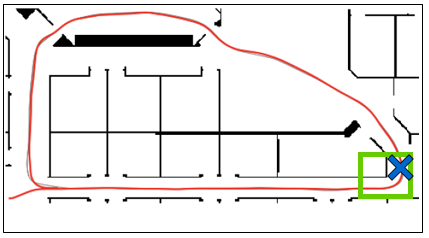
\includegraphics[keepaspectratio, scale=0.6]{images/result3.png}
  \caption{Failure point of the experiment2-2}
  \label{Fig:result3}
  \end{figure}

\paragraph{考察}
4000stepでは成功回数が0/10だったが, 8000step, 10000stepにすることで成功回数が1/10になり, 目標経路を一周することができた. このことから, 訓練する際に異常データから受ける影響が少なくて済むバッチ学習を用いて, 学習量を増やすことで成功回数が増えることを示せた. また, \figref{Fig:result3}の緑枠内の角で曲がりきれず, 青×に示す箇所でコースアウトしたが, 訓練2-1と比べて角で曲がる挙動が見られた. よって, 訓練2-2では成功回数が十分であるとは言えず, 角を曲がり切れていない. そこで, \figref{Fig:result3}の緑枠内のデータを水増しすることで角を曲がり切ることができ, 成功回数が増えるのではないかと考えた. 

\subsection{訓練2-3}
ここでは, 角のデータを水増しすることで成功回数が増えるかどうか検証する. 

\paragraph{訓練}
バッチサイズはデータ量と同じ8154, バッチ学習で4000step, 8000stp, 10000step学習した. 

\subsection{実験2-3}

\paragraph{実験結果}
実験結果は, \ref{tb:exp4}のようになった. 

\begin{table}[h]
  \centering
  \begin{tabular}{|c|c|} \hline
    step & Number of successes \\ \hline
    4000 & 0/10 \\ \hline
    8000 & 1/10 \\ \hline
    10000 & /10 \\ \hline
  \end{tabular}
  \caption{Number of successes in the experiment2-3}
  \label{tb:exp4}
\end{table}